\chapter{Data Collection}

\section{General Data Requirements}
Creating a quiz requires meticulous data collection and a clear understanding of the requirements to ensure that the questions generated are relevant, challenging, and beneficial for users.

\begin{enumerate}
    \customitem{Data Quality and Validation}
        \begin{enumerate}[label*=\arabic*.]
            \item Accuracy: Ensure the correctness of the data collected.
            \item Relevance: The data must be pertinent to the topics covered.
            \item Completeness: All necessary data points should be collected to generate comprehensive questions.
            \item Consistency: Standardize the format and structure of data for uniformity.
            \item Verification: Cross-check data with multiple sources and validate through SMEs.
        \end{enumerate}
\end{enumerate}



\subsection{Question generation data schema}
To effectively generate and manage quiz questions, a well-defined schema is essential. Below is a detailed schema that aligns with the requirements provided. This schema includes fields for context, difficulty level, question type, the question itself, choices (for MCQs), and the answer.

\newpage
\section*{Data Schema Overview}

\begin{enumerate}

    \item[Context] 
    \begin{description}[leftmargin=2em]
        \item[Description:] The reference or source from which the question is derived. This must cover a diversity of topics to ensure a broad range of subjects.
        \item[Type:] String
    \end{description}
    
    \item[Level] 
    \begin{description}[leftmargin=2em]
        \item[Description:] Indicates the difficulty level of the question.
        \item[Type:] Enum (hard, medium, easy)
    \end{description}
    
    \item[Type] 
    \begin{description}[leftmargin=2em]
        \item[Description:] Specifies the format of the question.
        \item[Type:] Enum (MCQ, Bool, Open)
    \end{description}
    
    \item[Question] 
    \begin{description}[leftmargin=2em]
        \item[Description:] The actual question text.
        \item[Type:] String
    \end{description}
    
    \item[Choices] 
    \begin{description}[leftmargin=2em]
        \item[Description:] Possible answers for Multiple Choice Questions (MCQs).
        \item[Type:] Array of Strings
        \item[Note:] This field is required only if the \textbf{Type} is "MCQ".
    \end{description}
    
    \item[Answer] 
    \begin{description}[leftmargin=2em]
        \item[Description:] The correct answer to the question.
        \item[Type:] String
        \item[Example:] "To declare a block-scoped variable"
        \item[Note:] The format may vary depending on the \textbf{Type} of question.
    \end{description}

\end{enumerate}

\newpage
\section*{Schema Definition}

Here is the schema definition in JSON format:

\begin{figure}[h!]
	\centering
	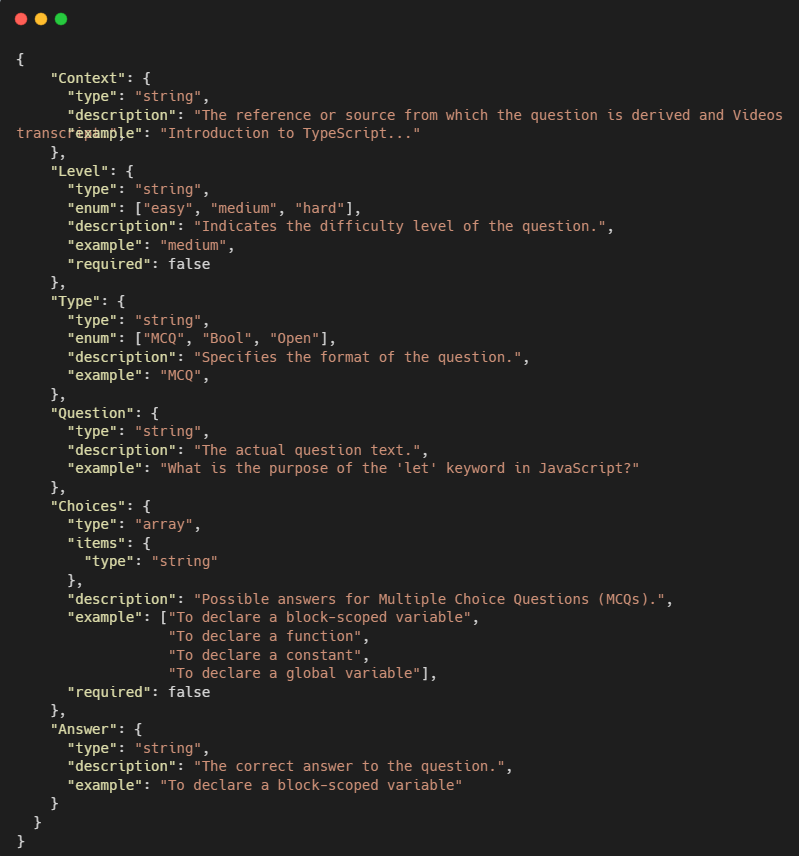
\includegraphics[scale=0.85]{figures/schema definition in JSON format.png}
	\caption{ Schema of data in json format }
\end{figure}


\begin{center}

\subsection*{Example Entries}

\subsection*{Multiple Choice Question (MCQ)}

\begin{verbatim}
{
  "Context": "This is the Human Papilloma Virus, which causes a viral STI. Viral STIs can be especially dangerous, as they cannot be cured. Once you get one, it's yours for life. And also, it's the person's you give it to.",
  "Type": "MCQ",
  "Question": "What makes viral stis more dangerous than other types?",
  "Choices": [
    "A. Jim.",
    "B. Steven.",
    "C. Green.",
    "D. Tom."
  ],
  "Answer": "B"
}
\end{verbatim}

\subsection*{True/False Question}

\begin{verbatim}
{
  "Context": " AR-15s in California The Roberti-Roos Assault Weapons Control Act of 1989 banned Colt AR-15 rifles by name in the State of California. California's 2000 Assault Weapons ban went further and banned AR-15s made by other manufacturers by name such as Bushmaster, PWA, and Olympic Arms.",
  "Type": "bool",
  "Question": "is it legal to own an ar15 in california.",
  "Answer": "false"
}
\end{verbatim}

\subsection*{Written Question}

\begin{verbatim}
{
  "Context": "Dan Dierdorf, 1974 to 1978 seasons: From 1974 to 1976, Dierdorf started every game at right tackle for the Cardinals during a three-year span in which the team compiled records of 10-4, 11-3, and 10-4 under head coach Don Coryell. In 1977, Dierdorf sustained a broken jaw and missed two games to injury as the Cardinals fell to 7-7.",
  "Type": "open",
  "Question": "What position did he play?",
  "Answer": "Dierdorf started every game at right tackle."
}
\end{verbatim}

\end{center}


\newpage

\subsection{Datasets}

\begin{description}
    \item[QUAC-CQA \cite{anantha2020open}] 
    \begin{description}[leftmargin=2em]
        \item[Location:] Local
        \item[Type:] Open
        \item[Size:] 74,977 examples
        \item[Link:] \url{https://huggingface.co/datasets/tilyupo/quac_cqa?row=4}
    \end{description}
    
    \item[RACE (Hugging Face)]
    \begin{description}[leftmargin=2em]
        \item[Location:] Hosted
        \item[Type:] MCQ
        \item[Size:] 195,374 examples
        \item[Description:] Collected from English exams for Chinese students aged 12 to 18, covering diverse topics.
        \item[Link:] \url{https://huggingface.co/datasets/race?row=26}
    \end{description}
    
    \item[SQuAD (Hugging Face) \cite{rajpurkar2016squad}]
    \begin{description}[leftmargin=2em]
        \item[Location:] Hosted
        \item[Type:] Open
        \item[Size:] 98,169 examples
        \item[Description:] Collection of question-answer pairs derived from Wikipedia articles, allowing any sequence of tokens as correct answers.
        \item[Link:] \url{https://huggingface.co/datasets/squad?row=31}
    \end{description}
    
    \item[Boolean Questions \cite{clark2019boolq}(Google Research)]
    \begin{description}[leftmargin=2em]
        \item[Location:] Local
        \item[Type:] Boolean
        \item[Size:] 15,699 examples
        \item[Link:] \url{https://github.com/google-research-datasets/boolean-questions}
    \end{description}
    
    \item[XQuAD (Google DeepMind) \cite{artetxe2019cross}]
    \begin{description}[leftmargin=2em]
        \item[Location:] Local
        \item[Type:] Open
        \item[Description:] Subset of 240 paragraphs and 1190 QA pairs from SQuAD v1.1.
        \item[Link:] \url{https://github.com/google-deepmind/xquad}
    \end{description}
    
    \item[SciQ \cite{pedersen2020sciq} (AllenAI)]
    \begin{description}[leftmargin=2em]
        \item[Location:] Local
        \item[Type:] MCQ
        \item[Size:] 13,679 examples
        \item[Description:] Crowdsourced science exam questions covering Physics, Chemistry, and Biology.
        \item[Link:] \url{https://allenai.org/data/sciq}
    \end{description}
    
    \item[ClarQ \cite{kumar2020clarq} (Vaibhav4595)]
    \begin{description}[leftmargin=2em]
        \item[Location:] Local
        \item[Size:] 4GB
        \item[Link:] \url{https://github.com/vaibhav4595/ClarQ}
    \end{description}
\end{description}

\subsubsection{QA Schema Summary}

The QA schema includes the following components:
\begin{itemize}
    \item \textbf{Context:} The reference or source from which the question is derived.
    \item \textbf{Question Level:} Indicates the difficulty level (easy, medium, hard).
    \item \textbf{Question Type:} Specifies the format of the question (MCQ, Boolean, Open).
    \item \textbf{Question:} The actual question text.
    \item \textbf{Answer Choices:} Possible answers for MCQs.
    \item \textbf{Correct Answer:} The correct answer to the question.
\end{itemize}

\subsubsection{Dataset Statistics}

The datasets collectively contain a total of 398,199 examples, broken down as follows:
\begin{itemize}
    \item \textbf{MCQ Questions:} 209,053 examples
    \item \textbf{Open Questions:} 173,146 examples
    \item \textbf{Boolean Questions:} 16,000 examples
\end{itemize}

These datasets cover a wide range of topics and were collected from various sources, providing a comprehensive collection for question generation and answering tasks.

\newpage

\section{Text Summarization Requirements}

Text summarization involves specific requirements to ensure effective processing and generation of concise summaries. These requirements typically include:

\subsection{Text Summarization Dataset Requirements}

\begin{itemize}
    \item \textbf{Size}: Datasets should be sufficiently large to train robust models. For example:
    \item \textbf{Quality}: Summaries should be accurate and relevant to the original texts, ensuring meaningful abstraction.
    \item \textbf{Diversity}: Datasets should cover a wide range of topics and domains to generalize well.
\end{itemize}



\subsection*{Text Summarization Datasets}

\subsection*{CCDV Datasets}

\begin{itemize}
    \item \href{https://huggingface.co/datasets/ccdv/govreport-summarization?row=2}{Government Report Summarization}
    \begin{itemize}
        \item Location: hosted
        \item Size: 19,463 records
        \item Token Limit:  9,000 characters /  500 tokens
    \end{itemize}
    
    \item \href{https://huggingface.co/datasets/ccdv/pubmed-summarization?row=3}{PubMed Summarization}
    \begin{itemize}
        \item Location: hosted
        \item Size: 266,430 records
        \item Token Limit:  3,000 characters /  215 tokens
    \end{itemize}
    
    \item \href{https://huggingface.co/datasets/ccdv/arxiv-summarization}{ArXiv Summarization}
    \begin{itemize}
        \item Location: hosted
        \item Size: 215,037 records
        \item Token Limit:  6,000 characters /  300 tokens
    \end{itemize}
\end{itemize}
